\documentclass{vldb}
\usepackage{url}
\usepackage{amsmath}
\usepackage{graphicx}
\usepackage{epstopdf}
\newcounter{ctResp}
\newcommand{\eat}[1]{}
\newcommand{\response}[1]{
\addtocounter{ctResp}{1}

\textbf{Response \arabic{ctResp}:} #1 \\}

\begin{document}
\title{Responses to reviewers' comments for Paper \# 278}
\maketitle

We are deeply grateful to all the reviewers for the 
%generous and 
insightful
suggestions which help us to improve this work.
In the following, we provide an explicit response to each concern raised.

\section{Response to Reviewer 1}

\textbf{1.1} \emph{The main con that I've spotted is the fact that the algorithm might have been
more nicely framed also within the Spark environment by taking advantage of
the various possibilities offered by it (e.g. caching of RDDs)}

\textbf{Response:} We agree with the reviewer that the solutions could benefit from utilizing advanced Spark features. 
In our previous submission, our SPARE algorithm has already
%In fact, our 
%the SPARE algorithm has already 
taken advantage of two distinct features of Spark, including  DAG execution engine and in-memory caching, to accelerate its performance:\\
\noindent\textbf{DAG Execution Engine:} As described in Section 5.3, our SPARE algorithm uses a run-time best-fit strategy to achieve load balance. This strategy relies on the DAG execution engine, which is a distinct feature of Spark. The strategy can be viewed as a planning phase in the Map-Planning-Reduce workflow. In particular, after the Map phase, we can collect the sizes of all stars as input for better workload balance among the reducers. Whereas, there is no such a planning phase in Hadoop. \\
\noindent\textbf{In-memory Caching:} We also utilize the in-memory caching feature of Spark to store the map result (i.e., RDDs of stars)
during the planning phase and reuse them in the reduce phase (Section 5.3). Such a caching feature is not available in Hadoop neither.

In our revision, we have edited Section 5.3 to explicitly clarify these points. Nevertheless, we believe there could exist other nice features of Spark worth further explorations in our solutions. 

\section{Response to Review 2}

\textbf{2.1} \emph{The GCMP generalization is not particularly novel. Putting a maximum gap size
on consecutive segments is well-known
in sequence mining published more than
10 years ago.}

\textbf{Response:} The idea of introducing a maximum gap size is indeed a commonly used method in sequence mining. However, 
it has not been employed in trajectory co-movement mining to resolve the loose-connection anomaly. More importantly, incorporating
this feature poses new challenges and we propose two types of efficient and scalable solutions for the more generalized problem.

To summarize, the novelty of the paper includes:
\begin{itemize}
\item We are the first to incorporate the parameter of maximum gap in the co-movement pattern definition. This has made
it possible to achieve our GCMP generalization. Such a generalization is more practical as it offers a single solution  
for a class of co-movement patterns, in contrast to specialized solutions for each class of patterns.

\item We are the first to deploy a distributed solution framework on Spark to solve the generalized pattern mining problem.
This enables large-scale (in terms of number of objects and trajectory duration) co-movement pattern mining to be accomplished
in a short time (in contrast to days in traditional centralized solutions).

\item There are also several novel ideas in our SPARE algorithm. For example, we devise a novel Star Partitioning to minimize data replication and a run-time best-fit strategy to achieve better workload balance. 
In order to apply Apriori algorithm to overcome the exponential enumeration problem, we also devise a  novel concept of sequence simplification to find a new type of monotonicity which can significantly reduce the number of candidates. This further renders our approach practical on large-scale datasets.
\end{itemize}


\textbf{2.2} \emph{In fact, I have doubts about formulating the GCMP patterns as proposed. Are
we really interested in all sets of movements beyond a cardinality of size $M$? 
Take the Taxi dataset as an example. Let say that there are lots of taxis going
from the airport to downtown. Let say that there are 1000 such taxis. For a
given $M$, are we interested in ${1000 \choose M}$ answers? 
So this speaks to the problem of picking $M$. If $M$ is 500, what is ${1000 \choose M}$? In fact, even if the
system gives the single answer of ${1000\choose 1000}$,
I am not sure I am
interested in this pattern as I already know that there are many taxis going from
the airport to downtown. What I think I am really interested in are GCMP that
are ``anomalous'', which is much harder to define.}

\textbf{Response:} We understand the reviewer's concern and we will respond to this issue from several aspects. First, in this example, the reviewer actually has the prior knowledge that there are lots of taxis going from airport to downtown. Hence, the results from the co-movement patterns may not look so interesting. If we consider another application in which the database contains the trajectories of all the citizens and our goal is to mine social relationships among them (i.e. friends may exhibit co-movement patterns), setting a proper $M$ becomes quite interesting and challenging. This is normally solved in an interactive way as in this case we don't have any prior knowledge. Second, it is possible that when $M$ is not set properly, an enormous number of ``valid'' patterns will be returned, as noticed by the reviewer. To solve this problem, a typical way is to use the concept of ``closed'' pattern, in which only the valid superset is returned. This can be seen as an incremental post-processing over our solution. Finally, we want to stress that we simply follow the definitions of co-movement patterns that are commonly adopted in the previous literature.



\textbf{2.3} \emph{Regarding the second weak points, one line of related work is the superimposition
of constraints on spatiotemporal mining. An example is a road network. In other words, given a road network, the network imposes constraints on GCMP.}

\textbf{Response:}
We agree with the reviewer that superimposition of constraints such as road network is an interesting research direction to consider. Despite many existing pattern discovery works in road networks~\cite{yu2016spatial,liu2013uncovering,liu2015exploring,xuTaxi2016}, we
are unaware of co-movement pattern works in the road context. 
In the future, we intend
to first formalize a new co-movement pattern with practically useful ``road-aware'' constraints, and then integrate the pattern discovery techniques
into our existing schemes. Meanwhile, we believe our work is able 
to attract more researchers to contribute to this field and inspire them
to consider advanced scenarios.
%
%Meanwhile, we believe our work is able to attract more researchers 
%to contribute to this field and to consider advanced scenarios.
%
%Therefore, 
%we believe co-movement patterns in the road networks is a potential interesting field and our
%work could 
%
%this work
%could attract more researchers' attention to contribute and consider more advanced scenarios. 
%In the future, we intend
%to formalize a new co-movement pattern with ``road-aware'' constraints, and to integrate the pattern discovery using our existing schemes.
%%
%%for our future work. 
%There are quite a few works that on discovers trajectory patterns in road networks~\cite{}. Currently, we are unaware of co-movement pattern queries in existing works, which However, we believe our work could attract other researchers' attention to contribute and consider more advanced scenarios. Further, we are also interested in explore co-movement patterns with ``road-aware-constraint'' in the future.

%In this paper, our goal is to first propose a unified definition of co-movement pattern that can generalize many previous works, and then design two scalable frameworks on Spark to solve this fundamental and general problem. We believe such a work can also attract other researchers' attention to contribute and consider more advanced scenarios with superimposition
%of constraints on spatiotemporal mining, as suggested by the reviewer.




%%%%%%%%%%%%%%%%%%%%%%%%%%%%%%%%%%%%%%%%%%%%%%%%%%%%%%%%%%%%%%%%%%%%%%%%%%%%%%%%%%%%%%%%%%
%%%%%%%%%%%%%%%%%%%%%%%%%%%%%%%%%%%%%%%%%%%%%%%%%%%%%%%%%%%%%%%%%%%%%%%%%%%%%%%%%%%%%%%%%%
%%%%%%%%%%%%%%%%%%%%%%%%%%%%%%%%%%%%%%%%%%%%%%%%%%%%%%%%%%%%%%%%%%%%%%%%%%%%%%%%%%%%%%%%%%

\section{Responses to Reviewer 3}
\textbf{3.1:} \emph{Though the implementation references Spark as the implementation
platform (as it also reflects in github repo provided), the algorithm design is
mostly limited to MapReduce, aka only Hadoop, which is a very small subset of
Spark. This may have a negative impact on the baseline implementation.
Particularly, recent releases of Spark have introduced window functions that can
be applied directly in the sliding window scenario here. Certainly, the algorithm
has to be redesigned to use DataFrame (and/or Spark SQL) interface, it has
been noted that this is a very efficient way to execute window functions in
Spark.}


\textbf{Response:} We thank the reviewer for the constructive comment.
% and carefully considered if applying the window-based function in the baseline algorithm is feasible.  
In our original submission,
we do not implement TRPM using Spark-SQL
because the latest Spark at that time (i.e., version 1.6.2 released in June)
did not support \textit{user defined aggregate function} (UDAF) on the window operator\footnote{Window function improvements: \url{https://issues.apache.org/jira/browse/SPARK-7712}}. 
Without UDAF, we cannot integrate the Line Sweep Mining (Algorithm 1) with the window functions. 
Following the release of Spark 2.0.0 which supports UDAF, we have now explored implementing TRPM using Spark-SQL window functions.

We construct a Spark-SQL query for TRPM (referred to as TRPM-SQL) in three steps:
First, we reorganize the input to form a Dataset\footnote{In Spark 2.0.0, Dataset is used to replace DataFrame.} with two columns: ``Time'' and ``Clusters''. 
Second, we create a WindowSpec to represent the sliding window with size $\eta$ on the ``Time'' column.
Last, we apply the WindowSpec and our Line Sweep Mining Algorithm (as UDAF) on the input Dataset.
%we call the window function in Spark-SQL with a UDAF representing our Line Sweep Algorithm. 
We compare the performance of TRPM-SQL with our original solutions in the following figure.
%
%Second, we extend the UDAF class to implement the Line Sweep Mining algorithm on the ``Clusters'' column. Third, we 
%create a WindowSpec to represent a sliding window with size $\eta$ on the ``Time'' column. We compare the performance
%of original Map-Reduce based TRPM (named TRPM-MR) with the TRMP-SQL in the following figure.

\begin{figure}[h]
\centering
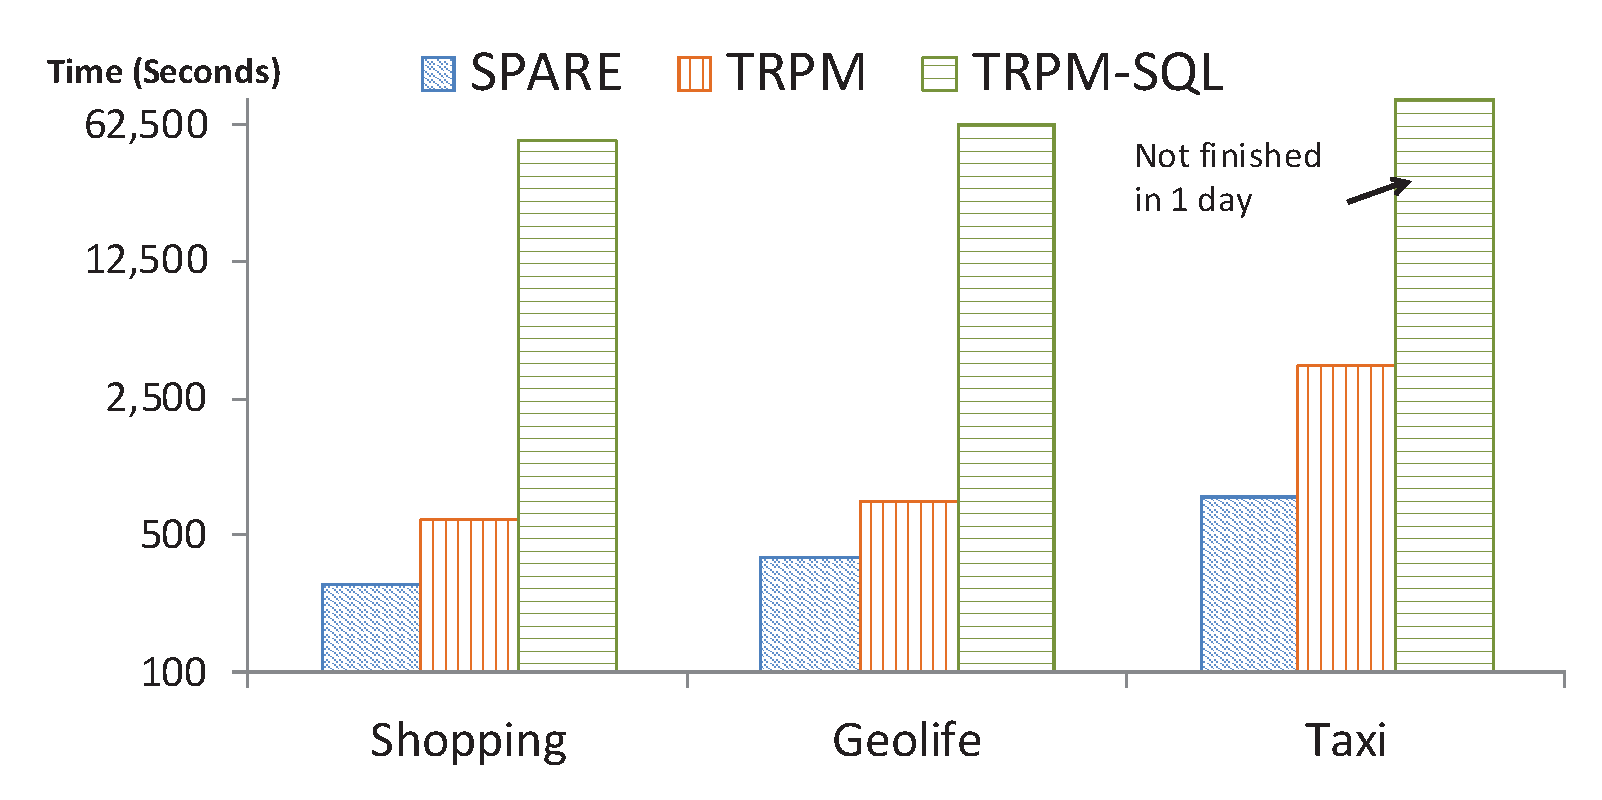
\includegraphics[width=0.4\textwidth]{spark-sql-comp.eps}
\caption{Performance comparison with SPARE, TRPM and TRPM-SQL}
\end{figure}

The figure clearly shows that TRPM-SQL is inefficient with over
120 times slower than TRPM. Our investigations on the query execution
plan identifies the root cause of  TRPM-SQL's slow performance to be the Spark-SQL Catalyst optimizer.
Since our TRPM-SQL query does not have a ``partition by'' clause, the Catalyst optimizer
treats the entire dataset as a SINGLE partition. Then it assigns the SINGLE partition to only ONE executor,
which fails to benefit from the parallelism of the Spark framework. 
Due to the inefficiency of TRPM-SQL (in Spark version 2.0.0), 
we do not use it to replace the baseline (i.e., TRPM). 
In our revision, we have added a footnote in Section 6 to justify our choice of implementations.



\textbf{3.2:} \emph{Most implementations
on Hadoop and Spark are very sensitive to data partitions, i.e. prone to data
skewing issues. It seems that the (starpartition)
implementation does not take
this into account, and only use the default partitioning. It would be very helpful
to have a discussion on this topic.}

\textbf{Response:} In our original submission, we actually have studied the skewness issue. In Section 5.3, we proposed a best-fit strategy for SPARE to achieve a better workload balance among the reducers because star partitioning may result in partitions with a different number of vertices. In the experimental study in Section 6.2.2, we have compared the SPARE algorithm with SPARE-RD and the latter only adopts the default random partition strategy. We presented the summary of the execution time for each method on the longest job and the standard deviation of all jobs in Table 9. The results show that SPARE demonstrates better load balance (lower deviation)
than SPARE-RD, which verifies the effectiveness of the best-fit strategy. 


\textbf{3.3:} \emph{In particular, it would be great to provide the
difference in the number of partitions/splits, the amount of processing and
memory usage (i.e., vcore and memory seconds) between TRPM and SPARE}

\textbf{Response:} We thank the reviewer for the suggestion and we have explicitly clarified these points in the revision.

In our implementation, we take a fixed 486 partitions (Section 6)
for each RDD. The partition number is determined according to
the parallel tuning guide by Cloudera\footnote{Spark Performance Tuning \url{http://blog.cloudera.com/blog/2015/03/how-to-tune-your-apache-spark-jobs-part-1/}}: there are  $3\times 54=162$ cores and each core is able to processes 3 partitions\footnote{This number may be different for other CPU models, and can be determined empirically.}
by multithreading.

Next, we have now added Table 7 (Section 6.1) to compare the resource usage between SPARE and TRPM in terms of Vcore-seconds and Memory. The results show that both SPARE and TRPM are resource efficient. In particular, the RDDs for both SPARE and TRPM only take less than 20\% of the available memory. This infers that SPARE and TRPM can handle
even larger trajectory databases with our current cluster resources.



\textbf{3.4:} \emph{A plot that breaks down the performance gain by each method would
be greatly appreciated by the readers.}

\textbf{Response:} We thank the reviewer for the advice. In the revision, we have added an analysis of
the breakdown cost in Figure 8. The SPARE and TRPM algorithms have similar workflow: partitioning (Star partition v.s. $\eta$-replicate partition) in the map-shuffle phase, and  mining (Apriori Enumeration v.s. Line Sweep) in the reduce phase. %In our experiment, we treat the execution time for each phase as the cost of the corresponding methods.
As shown in Figure 8,
both star partitioning and apriori enumeration contribute to 
the final performance gain of SPARE. Specifically, in the map-shuffle phase,
SPARE saves 56\%-73\% in time as compared to TRPM. This indicates that 
fewer data are replicated and shuffled in the star partitioning.
In the reduce phase, SPARE saves 46\%-81\% in time as compared to TRPM. This confirms 
the efficiency of our Apriori enumerator.

% with various optimization (e.g., sequence simplification, anti-monotonicity and forward closure checking).


\textbf{3.5} \emph{Some choices of words may need to be reconsidered: for example, ``a bunch
of" might not be appropriate in a technical paper.}

\textbf{Response:} We have changed these unprofessional terms.



\textbf{3.6} \emph{References to star partitioning and apriori pruning are missing. Though these
are well known, they need to  be clearly cited.}

\textbf{Response:} We have added the corresponding references in Section 5.1 and Section 5.2 when describing our algorithms.

\textbf{3.7} \emph{In ``In contrast, when utilizing the multicore
environment, SPAREP achieves 7 times speedup and SPARES achieves 10 times speedup.", was ``multicore"
referring to the use of all 16 cores in one of your node? The specification of the machine was not clear.}

\textbf{Response:} We used all cores in the single node (i.e., 4 executors each with 3 cores) to conduct the experiment. We have revised the description in Section 6.2.3.



\textbf{3.8} \emph{The computation of "eta" was slightly different than that in the paper}

\textbf{Response:} Thanks for pointing this out.  We have updated the GitHub repository to rectify the typo in the equation.


\section{Response to Meta Reviewer}

\textbf{M.1} \emph{Novelty: The GCMP generalization is not particularly novel. Please elaborate on the novelty of the work.}

\textbf{Response:} We have addressed this issue in Comment 2.1. 


\textbf{M.2} \emph{Parameter setting: Are we really interested in all sets of movements beyond a cardinality of size M? Please elaborate
on the motivation.}

\textbf{Response:} We have addressed this issue in Comment 2.2. 

\textbf{M.3} \emph{Spark implementation: the paper references Spark as the implementation platform but the algorithm is limited to MapReduce. Spark has capabilities beyond MapReduce such as window functions. Please provide an implementation that uses the relevant features of Spark, or a convincing discussion of how these features can be useful and why they were not used.}

\textbf{Response:} We have addressed this issue in Comments 1.1 and 3.1.

\textbf{M.4} \emph{More details in the performance evaluation: Please provide more details about data partitioning and the effect of skew. Also provide details about how star partitioning and a priori pruning contribute to performance. Please provide references to these two methods.}

\textbf{Response:} We have addressed these issues in Comments 3.2, 3.3, 3.4 and 3.6.

\bibliographystyle{IEEEtr}
\bibliography{citations}
\end{document}